\chapter{Einleitung}
Dies ist ein Minimalbeispiel für eine wissenschaftliche Arbeit an der Fakultät Informatik der \acrshort{hfu}.

\section{Abkürzungen}
\index{Abkürzung}
Abkürzungen werden in der Datei "glossary.tex" mit dem Befehl \mintinline{latex}{\newacronym} deklariert.
Im Text werden diese mit dem Befehl \mintinline{latex}{\gls} verwendet.

Beispielsweise kann die Abkürzung der Hochschule deklariert werden mit
\mint{latex}{\newacronym{hfu}{HFU}{Hochschule Furtwangen}}

Bei Erstverwendung es \mintinline{latex}{\gls} Befehls wird die volle Abkürzung ausgeschrieben, wie folgt:
\gls{hfu}.
Bei späterer Verwendung wird nur die Kurzform gedruckt: \gls{hfu}.

Soll eine spezifische Form der Abkürzung verwendet werden, gibt es noch die Befehle \mintinline{latex}{\acrfull}, \mintinline{latex}{\acrshort} und \mintinline{latex}{\acrlong}.

\section{Tabellen}
\index{Tabelle}
Tabellen werden in ein \mintinline{latex}{table}-Environment eingebettet.
Die Tabelle und Überschrift werden mit \mintinline{latex}{\centering} auf der Seite horizontal zentriert.
Die Überschrift wird mit \mintinline{latex}{\caption} über der Tabelle platziert.

Die Tabelle selbst wird mit einem \mintinline{latex}{tabular}-Environment angelegt.
Die verfügbaren Optionen für die Spaltenformattierungen des \mintinline{latex}{tabular}-Environments sind in \autoref{tab:table_options} aufgelistet.

\begin{table}
	\centering
	\caption{Verfügbare Optionen für die Spalten bei einer Tabelle}
	\label{tab:table_options}
	\begin{tabular}{ll}
		\toprule
		Option & Funktion \\
		\midrule
		l & linksbündig \\
		c & zentriert \\
		p\{breite\} & linksbündig mit fester Breite \\
		\bottomrule
	\end{tabular}
\end{table}

Horizontale Trennlinien lassen sich mit \mintinline{latex}{\toprule}, \mintinline{latex}{\midrule} und \mintinline{latex}{\bottomrule} setzen, entsprechend der Position.
Von vertikalen Trennlinien sollte abgesehen werden.

Die Zellen der Tabelle werden zeilenweise geschrieben.
Die Spalten werden mit \mintinline{latex}{&} getrennt, eine Zeile wird mit \mintinline{latex}{\\} abgeschlossen.

\section{Abbildungen}
\index{Abbildung}
Ähnlich wie Tabellen werden Abbildungen in das \mintinline{latex}{figure}-Environment eingebettet.
Ebenfalls wird die Abbildung mit Unterschrift durch den Befehl \mintinline{latex}{\centering} zentriert.

Die Abbildung selbst wird eingebunden mit 
\mint{latex}{\includegraphics[width=0.7\linewidth]{path/to/image}}
Die Unterschrift wird mit \mintinline{latex}{\caption} unter dem Bild platziert.

\begin{figure}
	\centering
	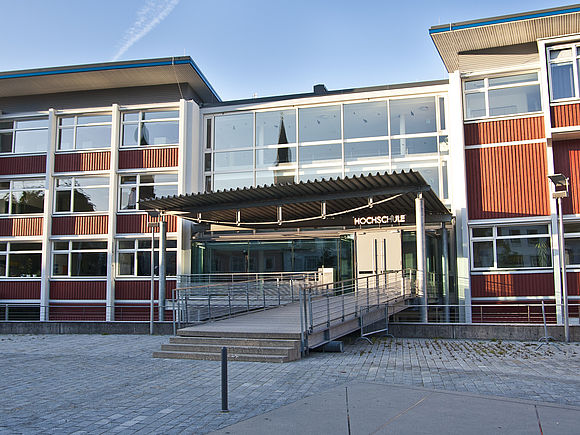
\includegraphics[width=0.7\linewidth]{content/pictures/hfu_a_bau}
	\caption{A-Bau der HFU, Campus Furtwangen}
	\label{fig:hfu_a_bau}
\end{figure}

\begin{wrapfigure}{r}{0.4\linewidth}
	\centering
	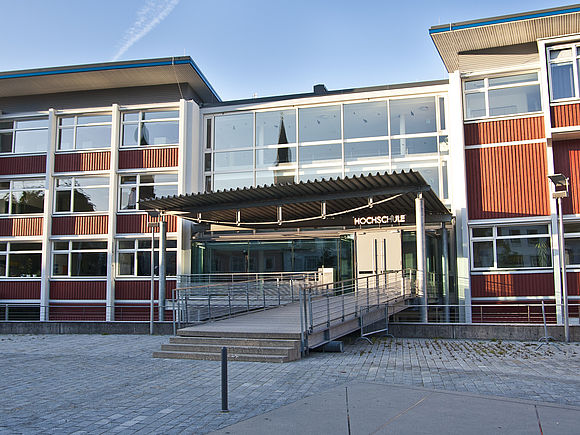
\includegraphics[width=0.8\linewidth]{content/pictures/hfu_a_bau}
	\caption{A-Bau der HFU, Campus Furtwangen}
	\label{fig:hfu_a_bau_wrap}
\end{wrapfigure}

\index{Abbildung!neben Text}
Alternativ kann eine Abbildung auch mit dem \mintinline{latex}{wrapfigure}-Environment neben dem Text platziert werden.
Dazu wird zusätzlich die Ausrichtung (\mintinline{latex}{l}/\mintinline{latex}{r}) und die Breite angegeben.

\section{Quellcode}
\index{Quellcode}
Quellcode kann in verschiedenen Formen eingebunden werden:

\begin{itemize}
	\item Inline
	\item Einzeiler
	\item Mehrzeiler
\end{itemize}

\index{Quellcode!inline}
Für inline-code wird der Befehl \mintinline{latex}{\mintinline{language}{code}} verwendet.
\index{Quellcode!einzeilig}
Analog wird für Einzeiler der Befehl
\mint{latex}{\mint{language}{code}}
verwendet.

\index{Quellcode!mehrzeilig}
Mehrzeiliger Quellcode wird in ein \mintinline{latex}{listing}-Environment eingebettet.
Die \mintinline{latex}{\caption} wird dabei unter dem Quellcode platziert.
Der Quellcode selbst wird inerhalb eines \mintinline{latex}{minted}-Environment geschrieben.
In \autoref{lis:multiline_code} ist beispielsweise der Code programmiert, der diese Ausgabe produziert.

\begin{listing}
\begin{minted}[linenos, tabsize=4]{latex}
\begin{listing}
	\begin{minted}[linenos, tabsize=4]{latex}
		...
	\end {minted}
	\caption{Multiline Quellcode}
	\label{lis:multiline_code}
\end{listing}
\end{minted}
\caption{Multiline Quellcode}
\label{lis:multiline_code}
\end{listing}

Zum Anzeigen von Zeilennummern wird die Option \mintinline{latex}{linenos} verwendet, zum Einstellen der Tab-Breite wird \mintinline{latex}{tabsize} spezifiziert.

\section{Referenzen}
\label{sec:references}
Textteile, Abbildungen, Tabellen und Quellcode kann im Text referenziert werden.
Dazu muss bei entsprechender Textstelle, Abbildung, Tabelle oder Quellcode mit \mintinline{latex}{\label{key}} ein Label gesetzt werden.
Dieses Label wird mit \mintinline{latex}{\ref{key}} referenziert.
Dabei wird die Aktuelle Kapitelnummer, Abbildungsnummer etc. angezeigt.

Für eine volle Referenz kann \mintinline{latex}{\autoref{key}} verwendet werden.
Bei einer Referenz auf den Aktuellen Abschnitt wird beispielsweise die Ausgabe "\autoref{sec:references}" erzeugt.

\section{Zitate}
Da dieses Thema umfangreicher ist sollte die Dokumentation von BibLaTeX herangezogen werden \parencite{biblatex}.
